\hsection{\crowsFoot{C}{O1}{D}{M1}}%
\label{sec:rm:cd}%
%
\begin{figure}%
\centering%
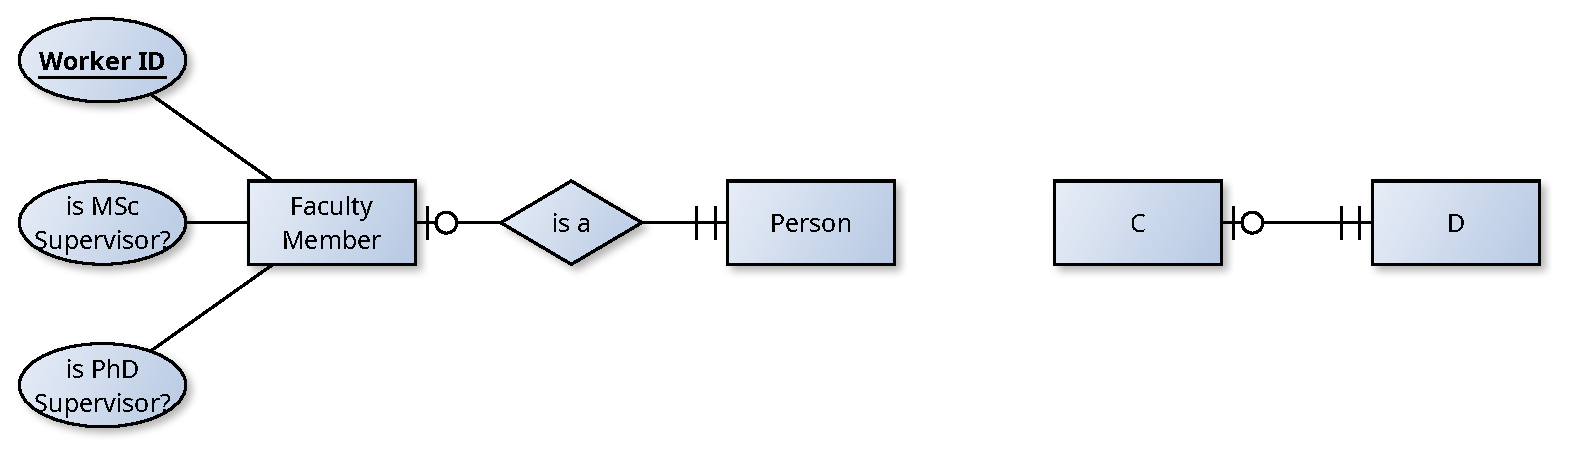
\includegraphics[width=0.97\linewidth]{\currentDir/CD}%
\caption{We encountered the \crowsFoot{C}{O1}{D}{M1} relationship pattern in \cref{fig:erdPersonStudentFaculty2}.}%
\label{fig:rm:cd}%
\end{figure}%
%
\gitLoadAndExecSQL{CD_tables}{}{conceptualToRelational}{CD_tables.sql}{relationships}{}{}%
\listingSQLandOutput{CD_tables}{%
The three-table realization of a \crowsFoot{C}{O1}{D}{M1} conceptual relationship.%
}{}%
%
\gitLoadAndExecSQL{CD_insert_and_select}{}{conceptualToRelational}{CD_insert_and_select.sql}{relationships}{}{}%
\listingSQLandOutput{CD_insert_and_select}{%
Inserting into and selecting data from the three-table realization of a \crowsFoot{C}{O1}{D}{M1} conceptual relationship given in \cref{lst:CD_tables}.%
}{}%
%
\gitExec{cdtrmTableC}{\databasesCodeRepo}{conceptualToRelational}{../_scripts_/db_table_to_latex_table.sh relationships c cid;fkdid;x}%
\gitExec{cdtrmTableD}{\databasesCodeRepo}{conceptualToRelational}{../_scripts_/db_table_to_latex_table.sh relationships d did;y}%
%
\begin{figure}%
\centering%
\floatSep%
\input{\gitFile{cdtrmTableC}}%
\floatSep%
\input{\gitFile{cdtrmTableD}}%
\floatSep%
\caption{The contents of the the tables in the implementation of the \crowsFoot{C}{O1}{D}{M1} conceptual relationship after executing \cref{lst:CD_insert_and_select}.}%
\label{fig:rm:cd:tables}%
\end{figure}%
%
\gitLoadAndExecSQL{CD_insert_error}{}{conceptualToRelational}{CD_insert_error.sql}{relationships}{}{}%
\listingSQLandOutput{CD_insert_error}{%
It is impossible to insert a row into table~\sqlil{c} that references a row in table~\sqlil{d} that is already referenced by another row in table~\sqlil{c}.%
}{}%
%
We have the two entity types~C and~D.
Each entity of type~C must be connected to exactly one entity of type~D.
Each entity of type~D is connected to zero or one entity of type~C.

We encountered this pattern when making a conceptual model of the relationship of persons, faculty, and students back in \cref{fig:erdPersonStudentFaculty2}.
In our conceptual model, each entity of type~\emph{Person} could be a~\emph{Faculty} or not.
Each entity of type \emph{Faculty} must be associated with one and exactly one record of type~\emph{Person}, as sketched in \cref{fig:rm:cd}.

The solution for implementing this in a \pgls{rdb} is similar to the two-table variant in the previous section:
We need a table~\sqlil{c} for the entities of type~C.
And we need a table~\sqlil{d} for the entities of type~D.
Both tables are also structured as in the previous section, including surrogate primary keys~\sqlil{cid} and~\sqlil{did} as well as attributes~\sqlil{x} and~\sqlil{y}, respectively.

Since each entity of type~C must be connected to exactly one entity of type~D, we add one column~\sqlil{fkdid} to the table for~C which holds the primary key to the D~entities as foreign key.
This column thus has a \sqlil{REFERENCES} constraint to the foreign key, which we add at the end of the script \cref{lst:CD_tables} via~\sqlil{ALTER TABLE}\sqlIdx{ALTER!TABLE}\sqlIdx{TABLE}.
Different from the previous section, this column~\sqlil{fkdid} must also have a \sqlil{NOT NULL}~constraint, because each entity of type~C must necessarily be related to one entity of type~D.
The column also has a \sqlil{UNIQUE} constraint, because the entities of type~D can only reference at most one entity of type~C.

We can only insert rows into the table for entity type~C that reference existing rows in the table for entity type~D.
The consequence is that these elements must be created first, as shown in~\cref{lst:CD_insert_and_select}.
Thus, after inserting data into table~\sqlil{d}, we then insert the rows into table~\sqlil{c}.
Each of these rows must provide a proper foreign key~\sqlil{fkdid} referencing the primary key~\sqlil{did} in table~\sqlil{d}.
The contents of the two tables~\sqlil{c} and~\sqlil{d} after executing \cref{lst:CD_insert_and_select} is illustrated in \cref{fig:rm:cd:tables}.
The data from the two tables can be combined using a single \sqlil{INNER JOIN}.

It is impossible to insert a row into table~\sqlil{c} that references a row in table~\sqlil{d} that is already referenced by another row in table~\sqlil{c}, as shown in \cref{lst:CD_insert_error}.
Neither can we insert a row into table~\sqlil{c} that does \emph{not} reference any row in table~\sqlil{d}, because of the \sqlil{NOT NULL} constraint, nor can we create a row in table~\sqlil{c} that references multiple rows in table~\sqlil{d}, since the foreign key attribute~\sqlil{fkdid} of table~\sqlil{c} can only take on one single value.
Notice that, together, this also means there can never be fewer entities of type~D than entities of type~C.%
%
\FloatBarrier%
\endhsection%
%
